% Options for packages loaded elsewhere
\PassOptionsToPackage{unicode}{hyperref}
\PassOptionsToPackage{hyphens}{url}
\PassOptionsToPackage{dvipsnames,svgnames,x11names}{xcolor}
%
\documentclass[
  10pt,
]{article}
\usepackage{amsmath,amssymb}
\usepackage{iftex}
\ifPDFTeX
  \usepackage[T1]{fontenc}
  \usepackage[utf8]{inputenc}
  \usepackage{textcomp} % provide euro and other symbols
\else % if luatex or xetex
  \usepackage{unicode-math} % this also loads fontspec
  \defaultfontfeatures{Scale=MatchLowercase}
  \defaultfontfeatures[\rmfamily]{Ligatures=TeX,Scale=1}
\fi
\usepackage{lmodern}
\ifPDFTeX\else
  % xetex/luatex font selection
\fi
% Use upquote if available, for straight quotes in verbatim environments
\IfFileExists{upquote.sty}{\usepackage{upquote}}{}
\IfFileExists{microtype.sty}{% use microtype if available
  \usepackage[]{microtype}
  \UseMicrotypeSet[protrusion]{basicmath} % disable protrusion for tt fonts
}{}
\makeatletter
\@ifundefined{KOMAClassName}{% if non-KOMA class
  \IfFileExists{parskip.sty}{%
    \usepackage{parskip}
  }{% else
    \setlength{\parindent}{0pt}
    \setlength{\parskip}{6pt plus 2pt minus 1pt}}
}{% if KOMA class
  \KOMAoptions{parskip=half}}
\makeatother
\usepackage{xcolor}
\usepackage[margin=0.7in]{geometry}
\usepackage{longtable,booktabs,array}
\usepackage{calc} % for calculating minipage widths
% Correct order of tables after \paragraph or \subparagraph
\usepackage{etoolbox}
\makeatletter
\patchcmd\longtable{\par}{\if@noskipsec\mbox{}\fi\par}{}{}
\makeatother
% Allow footnotes in longtable head/foot
\IfFileExists{footnotehyper.sty}{\usepackage{footnotehyper}}{\usepackage{footnote}}
\makesavenoteenv{longtable}
\usepackage{graphicx}
\makeatletter
\def\maxwidth{\ifdim\Gin@nat@width>\linewidth\linewidth\else\Gin@nat@width\fi}
\def\maxheight{\ifdim\Gin@nat@height>\textheight\textheight\else\Gin@nat@height\fi}
\makeatother
% Scale images if necessary, so that they will not overflow the page
% margins by default, and it is still possible to overwrite the defaults
% using explicit options in \includegraphics[width, height, ...]{}
\setkeys{Gin}{width=\maxwidth,height=\maxheight,keepaspectratio}
% Set default figure placement to htbp
\makeatletter
\def\fps@figure{htbp}
\makeatother
\setlength{\emergencystretch}{3em} % prevent overfull lines
\providecommand{\tightlist}{%
  \setlength{\itemsep}{0pt}\setlength{\parskip}{0pt}}
\setcounter{secnumdepth}{-\maxdimen} % remove section numbering
\ifLuaTeX
  \usepackage{selnolig}  % disable illegal ligatures
\fi
\usepackage{bookmark}
\IfFileExists{xurl.sty}{\usepackage{xurl}}{} % add URL line breaks if available
\urlstyle{same}
\hypersetup{
  colorlinks=true,
  linkcolor={Maroon},
  filecolor={Maroon},
  citecolor={Blue},
  urlcolor={blue},
  pdfcreator={LaTeX via pandoc}}

\author{}
\date{}

\begin{document}

\section{The special-fiber norm equations force the
origin}\label{the-special-fiber-norm-equations-force-the-origin}

2026-11-13. Source freeze
\texttt{5e342cafb852fe15d8744969dbd6de04f3561e77}; literal-issuer
correction \texttt{aec2bb861}. All claims unsigned {[}pcc:unverified{]}.

The explicit pole-scaled norm/membership family now has a Lean
implication: at parameter zero and Dickson depth4, vanishing of the four
nonconstant remainder coefficients forces \texttt{a1=a2=c0=c1=0}. The
result holds over every field, including extension fields. The family at
parameter one recovers the original symbolic target-completed norm
quotient and Dickson master. This establishes a precise zero-set fact
for the explicit family; its use as the actual reduced input's weighted
initial system still needs a faithful coefficient/filtration binding
{[}pcc:unverified{]}.

Central claim: \texttt{PCC-20261113-7b7707}.
\href{../lean/NormWeightedLeading.lean}{Proof source},
\href{../WEIGHTED_LEADING_PROTOCOL.md}{protocol},
\href{../weighted-leading-evidence/claim-pins.json}{claim map},
\href{special-fiber.dot}{editable diagram},
\href{special-fiber.svg}{SVG}, \href{report.pdf}{PDF}.

\begin{figure}
\centering
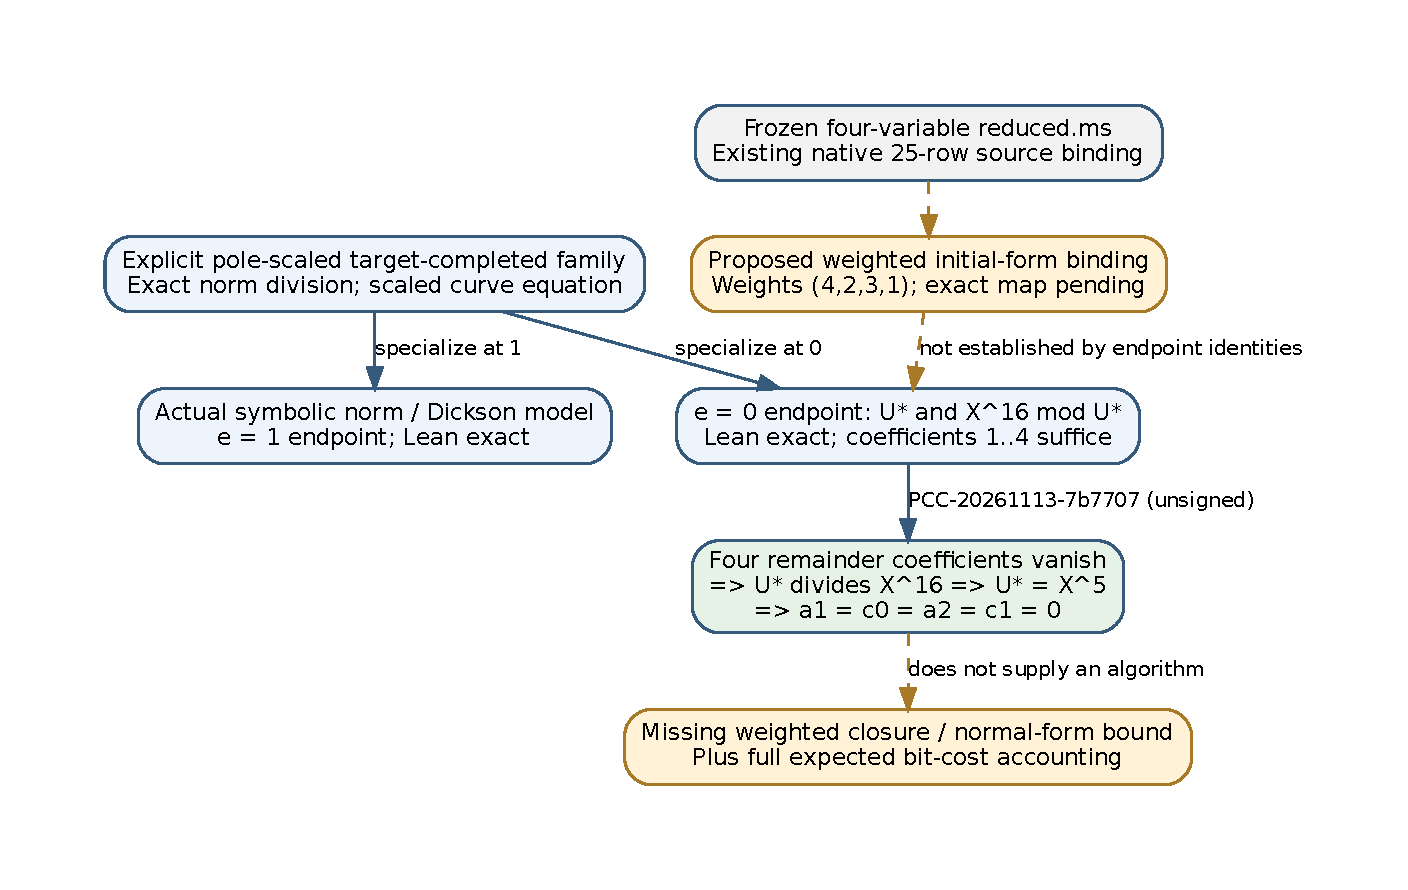
\includegraphics[width=0.9\textwidth,height=\textheight]{special-fiber.pdf}
\caption{Constructed family endpoints and the still-proposed
initial-form bridge. Solid arrows correspond to Lean
endpoint/implication results; dashed arrows are unresolved. All evidence
is unsigned.}
\end{figure}

\subsection{Construction and readable
proof}\label{construction-and-readable-proof}

Use the retained coefficient order \texttt{(a1,a2,c0,c1)}, proposed pole
weights \texttt{(4,2,3,1)}, and X weight2. Put
\texttt{D=X\^{}3+a2*X\^{}2+a1*X}, \texttt{B=c0+c1*X}. For parameter e,
curve \texttt{f\_e=X\^{}3+e\^{}4*a*X+e\^{}6*b}, target
\texttt{(q\_e,z\_e)=(e\^{}2*r,e\^{}3*z)}, and original curve equation
\texttt{z\^{}2=r\^{}3+a*r+b}, the scaled target lies on \texttt{f\_e}.
Use the existing actual \texttt{completeTarget} operation:

\begin{verbatim}
A_e = D + (z_e*B(q_e)-D(q_e))
U_e = (A_e^2-f_e*B^2) div (X-q_e).
M_0 = X; M_(n+1) = M_n^2-2*e^(2^(n+2))
R_e,n = (M_n-terminal*e^(2^(n+1))) mod U_e.
\end{verbatim}

The norm division is exact. At e=1 these are the original symbolic norm
quotient and Dickson recurrence; at e=0 the exact norm identity gives

\begin{verbatim}
U* = X^5 +(2*a2-c1^2)*X^4 +(a2^2+2*a1-2*c0*c1)*X^3
     +(2*a1*a2-c0^2)*X^2 +a1^2*X
R_0,4 = X^16 mod U*.
\end{verbatim}

\texttt{U*} is monic of degree5 and has constant zero. The remainder has
degree below5; its constant is zero because both dividend and divisor
vanish at0. Thus its four nonconstant coefficient equations imply the
whole remainder is zero. Consequently \texttt{U*} divides
\texttt{X\^{}16}. The prime-power divisor theorem and monicity give
\texttt{U*=X\^{}5}. Comparing coefficients, first \texttt{a1\^{}2=0},
then \texttt{c0\^{}2=0}, then \texttt{a2\^{}2=0}, then
\texttt{c1\^{}2=0}. A field has no nonzero nilpotents, so all four
coefficients vanish. No characteristic restriction is needed. The actual
remainder criterion also has a converse at every exponent
n\textgreater=5 {[}pcc:unverified{]}.

At e=0 the curve equation is \texttt{y\^{}2=x\^{}3}. This endpoint is
used only for the coefficient equations; no elliptic-group transport
through it is asserted. The zero tuple of this special fiber is not a
recovered solution of the original parameter-one problem. No theorem
transports that tuple across the family, assumes flatness, proves
regularity or supplies an efficient finder. A weighted homogeneous
zero-set argument and a low weighted last-fall bound are distinct
obligations {[}pcc:unverified{]}.

\subsection{Checks, failures and experiment
boundary}\label{checks-failures-and-experiment-boundary}

The module has18 new statements. Build007 records standard foundations
\texttt{propext}, \texttt{Classical.choice}, \texttt{Quot.sound}. The
whole-study gate reports 304 statements and0 additional trusted uses,
exit0; import-inclusive fresh replay also exits0. Validation claim
\texttt{PCC-20261113-582ee7} binds the
\href{../weighted-leading-evidence/validation-001.json}{receipt} with
exact source/artifact hashes and preserved exits. The module uses
standard \texttt{import\ all} access to existing definitions; no earlier
mathematical source, checker, dependency pin or gate changed
{[}pcc:unverified{]}.

Literal certificate \texttt{IDC1h0e1e85cab8ff464b}, claim
\texttt{PCC-20261113-027206}, encodes only the literal special-fiber
norm expansion displayed above. The unchanged issuer/checker accepts32
statement-derived and16 extra points. It is unsigned and does not
certify the geometric implication, Lean execution, initial forms or a
solver. The first issuance rejected degree6: ordinary syntactic degree
is7, from \texttt{X\^{}3*(c1*X)\^{}2}. Its failed log/exit is retained
under \texttt{PCC-20261113-aea26a}; the correction changed no expression
or mathematical acceptance criterion {[}pcc:unverified{]}.

The adapter's22 canonical tests and format/build pass in the saved
receipts. Strict clippy records four
\texttt{chunks\_exact\_to\_as\_chunks} style failures in the unchanged
canonical SHA256 under Rust1.99.1. No suppression or canonical source
edit was made. Old source/evidence/claims remain intact
{[}pcc:unverified{]}.

The preceding projection's saved benchrec diagnostic remains1680
historical sparse-artifact issues across162 unchanged records. This
component changes no benchmark record, generator, progress or gate path;
the diagnostic is preserved rather than relabeled as a pass
{[}pcc:unverified{]}.

The fixed native fixture-to-leading-form experiment did \textbf{not}
run. Flow: planned1, attempted0, completed0, excluded0,
admission-blocked1. Checkpoint gate first required a resume; after
supplying it, upload transport was unavailable: no configured profile or
checkpoint token. Both failures remain. The tracked root resume belonged
to another study and was restored; this task's resume is saved under
\texttt{weighted-leading-evidence/}. No AWS/vault request, paid job,
F4/msolve, branch search or performance measurement occurred. Local Lean
proof checking and literal algebra certificate issuance are mathematical
construction, separate from that unlaunched experiment
{[}pcc:unverified{]}.

\subsection{Sources and next discriminating
obligations}\label{sources-and-next-discriminating-obligations}

Sources checked (KB): unavailable as already recorded. The bounded
direct fallback and precise URLs are in
\href{../weighted-leading-evidence/prior-search-receipt.json}{prior-search-receipt.json}.
Read ml-cryptanalysis at
\texttt{8020e131a1a3806531d695b6bc7586473802dada}: formal README and
actual Closure/VariableClosure Lean sources. Full iterated closure
permits multiplication of newly derived low-degree rows; static Macaulay
multiples alone do not establish its closure. Those existing
ordinary-degree results are not new weighted ECDLP bounds
{[}pcc:unverified{]}.

Read Faugere, Safey El Din, Verron, arXiv1412.7547v2, section3.2
equation11, Theorem12 and section4. Weighted bounds have
regularity/homogeneity/position hypotheses and add input degrees; they
do not automatically bound a solver by its maximum input degree. The
proposed weights are not reverse chain-divisible. Neither theorem is
applied to the concrete source here {[}pcc:unverified{]}.

\begin{enumerate}
\def\labelenumi{\arabic{enumi}.}
\tightlist
\item
  Prove the exact pole-normalization/filtration map, or complete the
  frozen symbolic fixture binding once checkpoint upload admission is
  available. The predicted residual weights24,26,28,30,30 remain
  predictions.
\item
  Establish a weighted normal-form/iterated-closure certificate with
  finite budgets. A low degree at one fixed fixture is not an asymptotic
  bound.
\item
  Prove a growing-family weighted last-fall bound and include
  decomposition yield, finite-field extraction, supplied-label relation
  collection and all expected bit costs. No generic regularity
  assumption fills this gap {[}pcc:unverified{]}.
\end{enumerate}

The original W-jet/rank proposal remains a separate family without a
faithful public map. No jet/rank attack or non-generic lower bound
follows here. Existing global scoreboard, timeline and curve diagrams
remain unchanged: this component has no new measured speed or certified
transport edge. The study-local diagram explicitly separates constructed
endpoints from the proposed weighted-initial-form bridge
{[}pcc:unverified{]}.

\subsection{Exact proof map}\label{exact-proof-map}

Every row has the exact field and parameter hypotheses in the linked
Lean declaration; the binding hash and source commit are in
claim-pins.json. All entries are unsigned {[}pcc:unverified{]}.

\begin{longtable}[]{@{}ll@{}}
\toprule\noalign{}
Lean declaration (namespace NormWeightedLeading) & Unsigned claim \\
\midrule\noalign{}
\endhead
\bottomrule\noalign{}
\endlastfoot
\texttt{monicDivisorPower} & \texttt{PCC-20261113-dc02f2} \\
\texttt{supportMonic} & \texttt{PCC-20261113-2bbd73} \\
\texttt{supportDegree} & \texttt{PCC-20261113-e3477f} \\
\texttt{supportPowerForcesZero} & \texttt{PCC-20261113-96dfec} \\
\texttt{supportDivisorForcesZero} & \texttt{PCC-20261113-2e2e93} \\
\texttt{supportRemainderForcesZero} & \texttt{PCC-20261113-c31867} \\
\texttt{supportRemainderIffZero} & \texttt{PCC-20261113-bbbc67} \\
\texttt{scaledCurveAtTarget} & \texttt{PCC-20261113-e562e9} \\
\texttt{leadingNormIdentity} & \texttt{PCC-20261113-fe03ff} \\
\texttt{scaledSupportZero} & \texttt{PCC-20261113-d4d4af} \\
\texttt{scaledSupportOne} & \texttt{PCC-20261113-677b73} \\
\texttt{scaledSupportExact} & \texttt{PCC-20261113-2868f3} \\
\texttt{scaledFiberRemainderForcesZero} &
\texttt{PCC-20261113-33be81} \\
\texttt{fourCoefficientsForceZero} & \texttt{PCC-20261113-06284b} \\
\texttt{scaledMasterZero} & \texttt{PCC-20261113-e00654} \\
\texttt{scaledMasterOne} & \texttt{PCC-20261113-2bcb8a} \\
\texttt{scaledMembershipZero} & \texttt{PCC-20261113-45c790} \\
\texttt{membershipFourCoefficients} & \texttt{PCC-20261113-7b7707} \\
\end{longtable}

\end{document}
